\documentclass{article}
\usepackage[utf8]{inputenc}
\usepackage{relsize}
\usepackage{amsmath}
\usepackage{geometry}
\usepackage{tikz}
\usetikzlibrary{automata, positioning, arrows}
\tikzset{node distance=2.5cm, % Minimum distance between two nodes. Change if necessary.
every state/.style={ % Sets the properties for each state
semithick,
fill=gray!10},
initial text={}, % No label on start arrow
double distance=2pt, % Adjust appearance of accept states
every edge/.style={ % Sets the properties for each transition
draw,->,>=stealth', % Makes edges directed with bold arrowheads
auto,semithick}}

\geometry{
 a4paper,
 total={170mm,257mm},
 left=20mm,
 top=20mm,
}

\title{Homework 2\\[0.2em]\smaller{}CSC 445-01: Theory of Computation}
\author{Matthew Mabrey, Luke Kurlandski}
\date{\today}

\begin{document}

\maketitle

\section*{1.4}
We use blue for 'b' and red for 'a' when space is limited

\section*{e}
$w$ starts with an 'a'
\begin{center}
    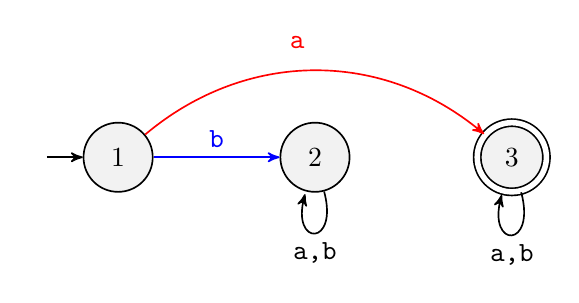
\begin{tikzpicture}
    
    \node[state, initial] (1) {$1$};
    \node[state, right of=1] (2) {$2$};
    \node[state, right of=2, accepting] (3) {$3$};
    
    \draw (1) edge[left, bend left=40, red] node[yshift=10pt, red] {\tt a} (3);
    \draw (1) edge[blue] node[blue] {\tt b} (2);
    
    \draw (2) edge[loop below] node {\tt a,b} (2);
    \draw (3) edge[loop below] node {\tt a,b} (3);
    
    \end{tikzpicture}
\end{center}
$w$ has at most one 'b'
\begin{center}
    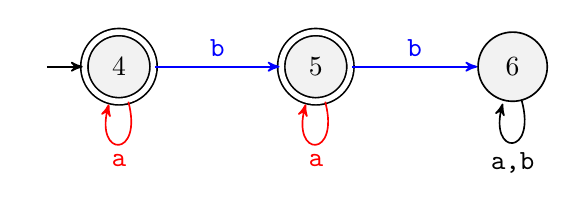
\begin{tikzpicture}
    
    \node[state, initial, accepting] (4) {$4$};
    \node[state, right of=4, accepting] (5) {$5$};
    \node[state, right of=5] (6) {$6$};
    
    \draw (4) edge[blue] node[blue] {\tt b} (5);
    \draw (5) edge[blue] node[blue] {\tt b} (6);
    
    \draw (4) edge[loop below, red] node[red] {\tt a} (4);
    \draw (5) edge[loop below, red] node[red] {\tt a} (5);
    \draw (6) edge[loop below] node {\tt a,b} (6);
    
    \end{tikzpicture}
\end{center}
$w$ starts with an 'a' and has at most one 'b'
\begin{center}
    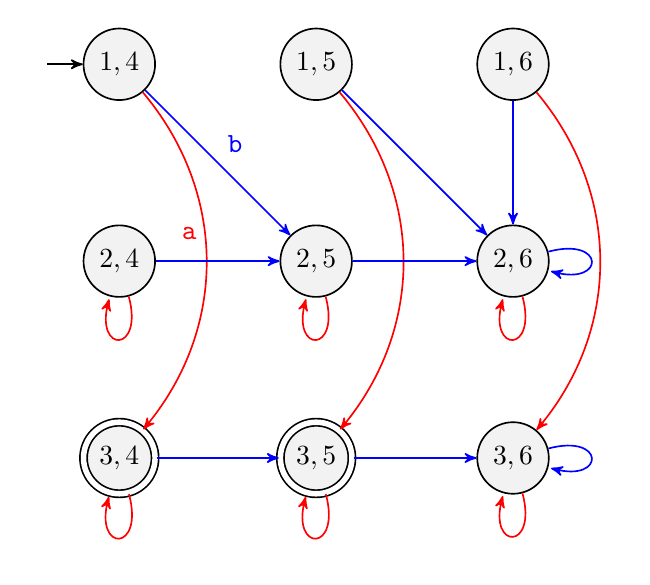
\begin{tikzpicture}
    
    \node[state, initial] (14) {$1,4$};
    \node[state, right of=14] (15) {$1,5$};
    \node[state, right of=15] (16) {$1,6$};
    \node[state, below of=14] (24) {$2,4$};
    \node[state, right of=24] (25) {$2,5$};
    \node[state, right of=25] (26) {$2,6$};
    \node[state, below of=24, accepting] (34) {$3,4$};
    \node[state, right of=34, accepting] (35) {$3,5$};
    \node[state, right of=35] (36) {$3,6$};
    
    \draw (14) edge[blue] node[blue] {\tt b} (25);
    \draw (14) edge[left, bend left=40, red] node[yshift=10pt] {\tt a} (34);
    \draw (15) edge[blue] node[blue] {\tt } (26);
    \draw (15) edge[left, bend left=40, red] node {\tt } (35);
    \draw (16) edge[blue] node[blue] {\tt } (26);
    \draw (16) edge[left, bend left=40, red] node {\tt } (36);
    
    \draw (24) edge[loop below, red] node[red] {\tt } (24);
    \draw (24) edge[blue] node[blue] {\tt } (25);
    \draw (25) edge[loop below, red] node[red] {\tt } (25);
    \draw (25) edge[blue] node[blue] {\tt } (26);
    \draw (26) edge[loop below, red] node[red] {\tt } (26);
    \draw (26) edge[loop right, blue] node[blue] {\tt } (26);
    
    \draw (34) edge[loop below, red] node[red] {\tt } (34);
    \draw (34) edge[blue] node[blue] {\tt } (35);
    \draw (35) edge[loop below, red] node[red] {\tt } (35);
    \draw (35) edge[blue] node[blue] {\tt } (36);
    \draw (36) edge[loop below, red] node[red] {\tt } (36);
    \draw (36) edge[loop right, blue] node[blue] {\tt } (36);
    
    \end{tikzpicture}
\end{center}
\pagebreak

\section*{f}
$w$ has an odd number of 'a'
\begin{center}
    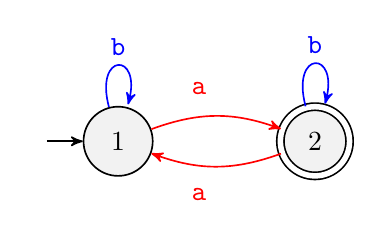
\begin{tikzpicture}
    
    \node[state, initial] (1) {$1$};
    \node[state, right of=1, accepting] (2) {$2$};
    
    \draw (1) edge[left, bend left=20, red] node[red, yshift=10] {\tt a} (2);
    \draw (2) edge[left, bend left=20, red] node[red, yshift=-10] {\tt a} (1);
    
    \draw (1) edge[loop above, blue] node[blue] {\tt b} (1);
    \draw (2) edge[loop above, blue] node[blue] {\tt b} (2);
    
    \end{tikzpicture}
\end{center}
$w$ ends in a 'b'
\begin{center}
    \begin{tikzpicture}
    
    \node[state, initial] (3) {$3$};
    \node[state, right of=3, accepting] (4) {$4$};
    
    \draw (3) edge[left, bend left=20, red] node[red, yshift=10] {\tt a} (4);
    \draw (4) edge[left, bend left=20, blue] node[blue, yshift=-10] {\tt b} (3);
    
    \draw (3) edge[loop above, red] node[red] {\tt a} (3);
    \draw (2) edge[loop above, blue] node[blue] {\tt b} (2);
    
    \end{tikzpicture}
\end{center}
$w$ has an odd number of 'a' and ends in a 'b'
\begin{center}
    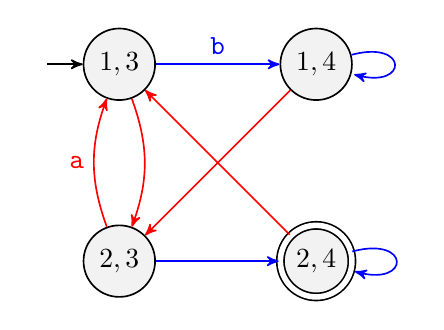
\begin{tikzpicture}
    
    \node[state, initial] (13) {$1,3$};
    \node[state, right of=13] (14) {$1,4$};
    \node[state, below of=13] (23) {$2,3$};
    \node[state, right of=23, accepting] (24) {$2,4$};
    
    \draw (13) edge[left, bend left=20, red] node[red] {\tt} (23);
    \draw (23) edge[left, bend left=20, red] node[red] {\tt a} (13);
    \draw (14) edge[red] node[red] {\tt} (23);
    \draw (24) edge[red] node[red] {\tt} (13);
    
    \draw (13) edge[blue] node[blue] {\tt b} (14);
    \draw (23) edge[blue] node[blue] {\tt} (24);
    \draw (14) edge[blue, loop right] node[blue] {\tt} (14);
    \draw (24) edge[blue, loop right] node[blue] {\tt} (24);
    
    \end{tikzpicture}
\end{center}

\section*{g}

$w$ has an even length
\begin{center}
    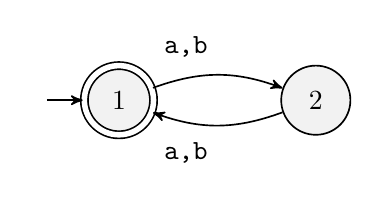
\begin{tikzpicture}
    
    \node[state, initial, accepting] (1) {$1$};
    \node[state, right of=1] (2) {$2$};
    
    \draw (1) edge[left, bend left=20] node[yshift=10] {\tt a,b} (2);
    \draw (2) edge[left, bend left=20] node[yshift=-10] {\tt a,b} (1);
    
    \end{tikzpicture}
\end{center}
$w$ has an odd number of 'a'
\begin{center}
    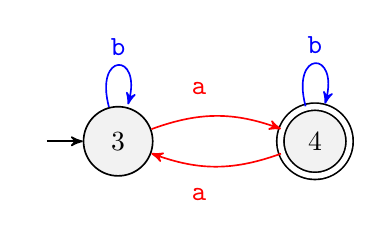
\begin{tikzpicture}
    
    \node[state, initial] (3) {$3$};
    \node[state, right of=3, accepting] (4) {$4$};
    
    \draw (3) edge[left, bend left=20, red] node[red, yshift=10] {\tt a} (4);
    \draw (4) edge[left, bend left=20, red] node[red, yshift=-10] {\tt a} (3);
    
    \draw (3) edge[loop above, blue] node[blue] {\tt b} (3);
    \draw (4) edge[loop above, blue] node[blue] {\tt b} (4);
    
    \end{tikzpicture}
\end{center}
$w$ has an even length and has an odd number of 'a'
\begin{center}
    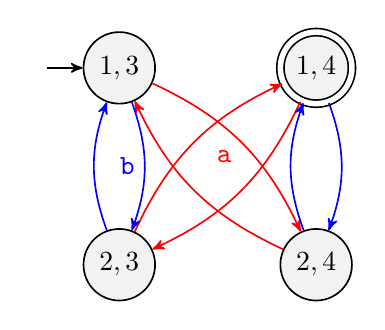
\begin{tikzpicture}
    
    \node[state, initial] (13) {$1,3$};
    \node[state, right of=13, accepting] (14) {$1,4$};
    \node[state, below of=13] (23) {$2,3$};
    \node[state, right of=23] (24) {$2,4$};
    
    \draw (13) edge[left, bend left=20, red] node[red, yshift=-5] {\tt a} (24);
    \draw (24) edge[left, bend left=20, red] node[red] {\tt} (13);
    \draw (23) edge[left, bend left=20, red] node[red] {\tt} (14);
    \draw (14) edge[left, bend left=20, red] node[red] {\tt} (23);
    
    \draw (13) edge[left, bend left=20, blue] node[blue] {\tt b} (23);
    \draw (23) edge[left, bend left=20, blue] node[blue] {\tt} (13);
    \draw (14) edge[left, bend left=20, blue] node[blue] {\tt} (24);
    \draw (24) edge[left, bend left=20, blue] node[blue] {\tt} (14);
    
    \end{tikzpicture}
\end{center}
\pagebreak

\section*{1.5}

\section*{g}

$w$ is any string that contains exactly two 'a'
\begin{center}
    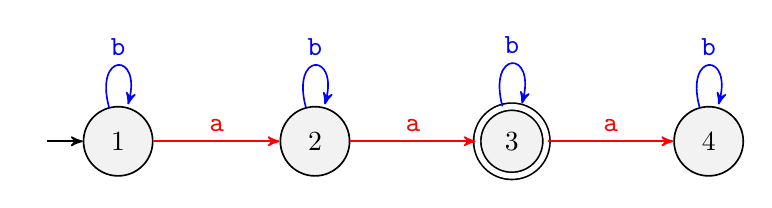
\begin{tikzpicture}
    
    \node[state, initial] (1) {$1$};
    \node[state, right of=1] (2) {$2$};
    \node[state, right of=2, accepting] (3) {$3$};
    \node[state, right of=3] (4) {$4$};
    
    \draw (1) edge[red] node[red] {\tt a} (2);
    \draw (2) edge[red] node[red] {\tt a} (3);
    \draw (3) edge[red] node[red] {\tt a} (4);
    
    \draw (1) edge[loop above, blue] node[blue] {\tt b} (1);
    \draw (2) edge[loop above, blue] node[blue] {\tt b} (2);
    \draw (3) edge[loop above, blue] node[blue] {\tt b} (3);
    \draw (4) edge[loop above, blue] node[blue] {\tt b} (4);
    
    \end{tikzpicture}
\end{center}
$w$ is any string that does not contain exactly two 'a'
\begin{center}
    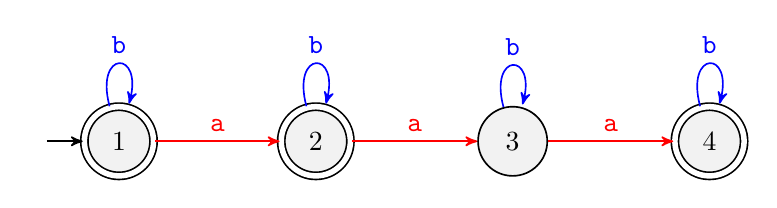
\begin{tikzpicture}
    
    \node[state, initial, accepting] (1) {$1$};
    \node[state, right of=1, accepting] (2) {$2$};
    \node[state, right of=2] (3) {$3$};
    \node[state, right of=3, accepting] (4) {$4$};
    
    \draw (1) edge[red] node[red] {\tt a} (2);
    \draw (2) edge[red] node[red] {\tt a} (3);
    \draw (3) edge[red] node[red] {\tt a} (4);
    
    \draw (1) edge[loop above, blue] node[blue] {\tt b} (1);
    \draw (2) edge[loop above, blue] node[blue] {\tt b} (2);
    \draw (3) edge[loop above, blue] node[blue] {\tt b} (3);
    \draw (4) edge[loop above, blue] node[blue] {\tt b} (4);
    
    \end{tikzpicture}
\end{center}

\section*{1.7}

\section*{b}

\section*{c}

\section*{e}

\section*{1.31}

\section*{1.33}

From problem 1.31, we know we are allowed to "wind the tape backwards" i.e., we will demonstrate that $C^R$ is a regular language, thus prove that $C$ itself is regular. To prove that $C^R$ is regular, we will construct a nondeterministic finite automata that recognizes $C^R$. \\\\
For each symbol, we will read its top bit and judge whether or not the bottom bit is correct such that $3 \textrm{row}_1 = \textrm{row}_2$. To do so, we track two conditions: 1) whether or not $3 \textrm{row}_1$ results in a carry-out in base two and 2) what the previous top symbol is. With these two pieces of information, given a top bit, we can check to see if the bottom bit is correct.\\\\
These two pieces of information result in an automata with 4 states to keep track of, but we had an additional start state.
\begin{itemize}
    \item $q_0$ : the start state, to prevent the automata from accepting the empty string
    \item $q_1$ : the state where there is no carry-in from previous step and the previous top symbol is a $0$
    \item $q_2$ : the state where there is a carry-in and the previous top value is a $1$
    \item $q_3$ : the state where there is no carry-in and the previous top value is a $1$
    \item $q_4$ : the state where there is a carry-in from previous step and the previous top value is a $0$
\end{itemize}
Our transition function merely
Recall that we read the string backwards, so the binary number is read from the $2^0$th place first. 
\begin{center}
    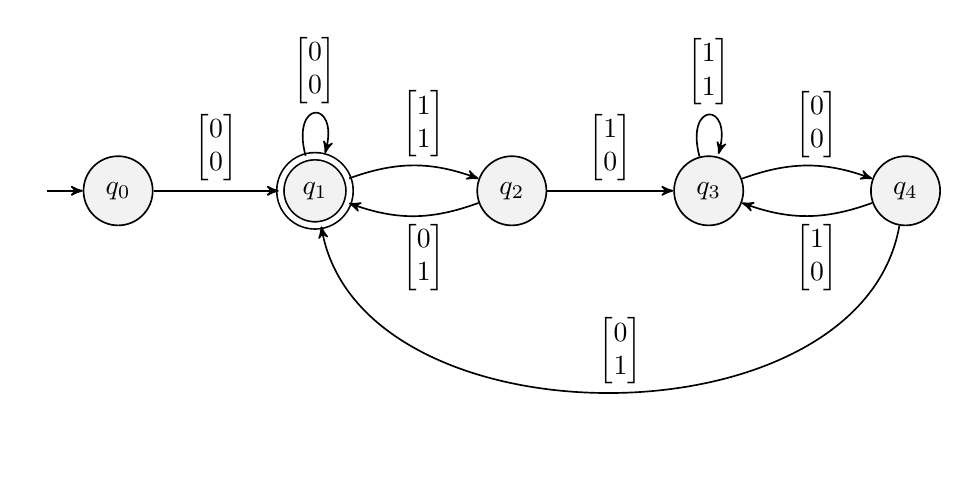
\begin{tikzpicture}
    
    \node[state, initial] (q0) {$q_0$};
    \node[state, right of=q0, accepting] (q1) {$q_1$};
    \node[state, right of=q1] (q2) {$q_2$};
    \node[state, right of=q2] (q3) {$q_3$};
    \node[state, right of=q3] (q4) {$q_4$};

    \draw (q0) edge node {\tt $\begin{bmatrix} 0 \\ 0 \end{bmatrix}$} (q1);
    \draw (q1) edge[loop above] node {\tt $\begin{bmatrix} 0 \\ 0 \end{bmatrix}$} (q1);
    \draw (q1) edge[left, bend left=20] node[xshift=15pt, yshift=15pt] {\tt $\begin{bmatrix} 1 \\ 1 \end{bmatrix}$} (q2);
    \draw (q2) edge[left, bend left=20] node[xshift=15pt, yshift=-15pt] {\tt $\begin{bmatrix} 0 \\ 1 \end{bmatrix}$} (q1);
    \draw (q2) edge node {\tt $\begin{bmatrix} 1 \\ 0 \end{bmatrix}$} (q3);
    \draw (q3) edge[loop above] node {\tt $\begin{bmatrix} 1 \\ 1 \end{bmatrix}$} (q3);
    \draw (q3) edge[left, bend left=20] node[xshift=15pt, yshift=15pt] {\tt $\begin{bmatrix} 0 \\ 0 \end{bmatrix}$} (q4);
    \draw (q4) edge[left, bend left=20] node[xshift=15pt, yshift=-15pt] {\tt $\begin{bmatrix} 1 \\ 0 \end{bmatrix}$} (q3);
    \draw (q4) edge[left, bend left=80] node[xshift=15pt, yshift=15pt] {\tt $\begin{bmatrix} 0 \\ 1 \end{bmatrix}$} (q1);
    
    \end{tikzpicture}
\end{center}

\section*{1.34}

\end{document}
